% Evidence and figure contracts: Analysis056/observations/001-paired-displacement.md.
% Queue the full-width figures before the empirical discussion.
\begin{figure*}[!t]
  \centering
  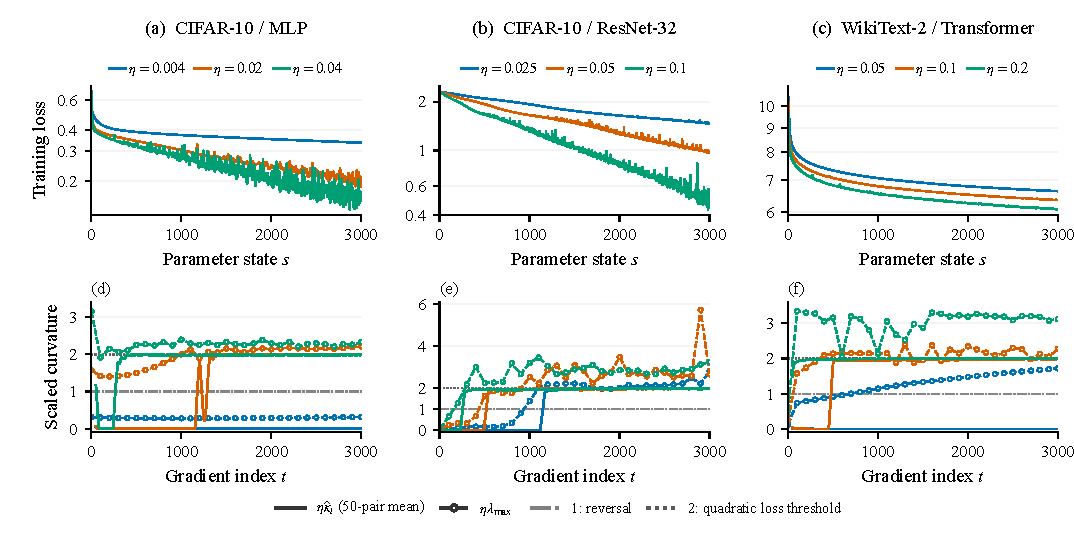
\includegraphics[width=\textwidth]{figures/analysis056/gd_loss_curvature.pdf}
  \caption{\textbf{Oscillatory loss reduction and directional curvature in GD.}
  Columns identify dataset/model; colors identify learning rate.
  Top: unsmoothed full-objective loss on logarithmic axes.
  Bottom: $\eta\widehat\kappa_t$ (solid, complete 50-pair trailing means)
  and recorded $\eta\lambda_{\max}$ (dashed with circles).
  Reference lines mark the alignment threshold at one and the
  quadratic-model loss-change threshold at two; their stepwise
  interpretation applies before smoothing.
  Spectra use the complete MLP objective, 5,000/50,000 ResNet images
  and 2,500/59,680 Transformer sequences. They are pointwise maxima;
  the secant is a directional path average under the smooth full-GD
  interpretation. Loss uses state $s$; a spectrum at state $s$ is
  placed at $t=s+2$, the starting state for $\widehat\kappa_t$.
  The final spectrum has no recorded gradient pair.}
  \label{fig:gd-loss}
\end{figure*}

\begin{figure*}[!t]
  \centering
  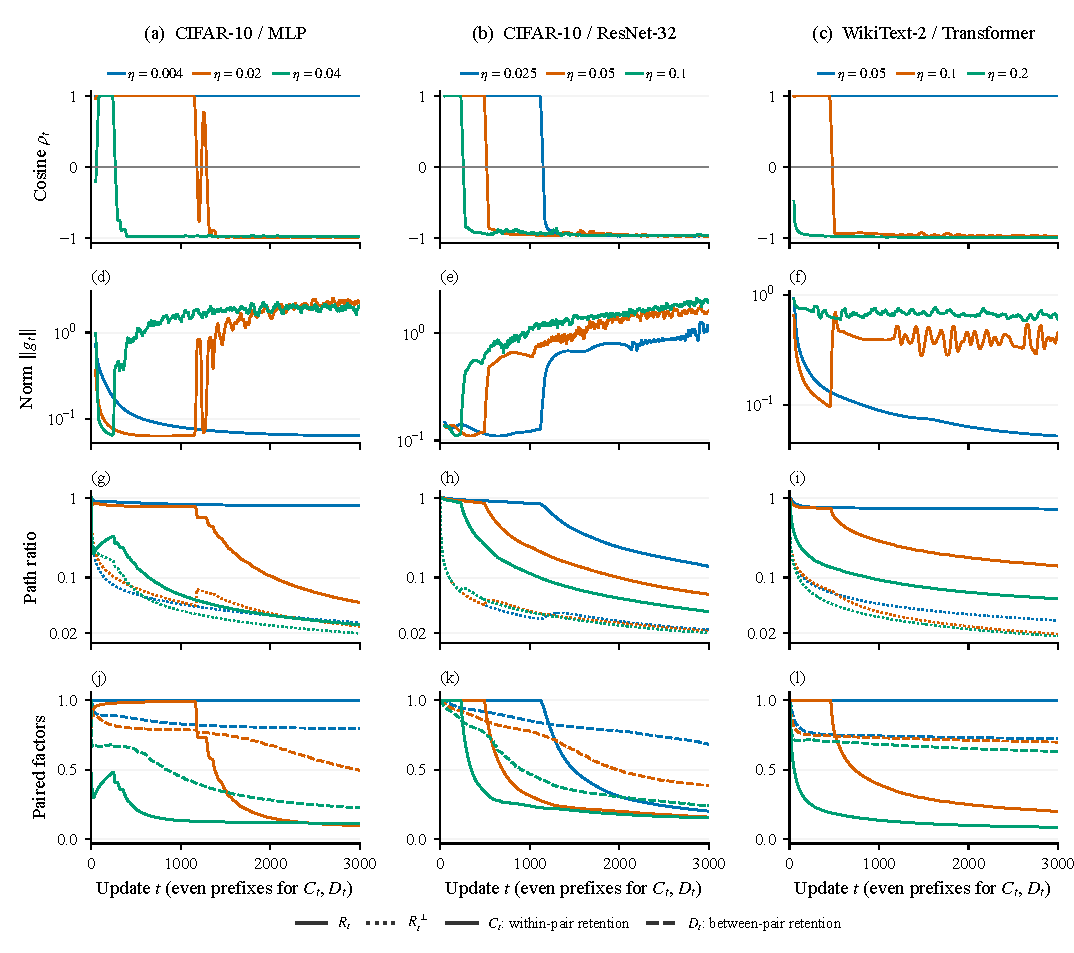
\includegraphics[width=\textwidth]{figures/analysis056/gd_reversal_paired_displacement.pdf}
  \caption{\textbf{Local reversal, cumulative displacement and paired motion.}
  Rows show consecutive cosine, gradient norm (log scale), $R_t$ with
  its zero-cross-term reference $R_t^{\perp}$ (log scale), and the
  factors $C_t$ and $D_t$ in Eq.~\eqref{eq:paired-displacement}.
  Cosines and norms use complete 50-observation trailing means;
  ratios use raw prefix sums, with paired factors at every even prefix.
  Colors denote the same rates as Fig.~\ref{fig:gd-loss}.
  At the largest rates, $R_{3000}$ is 2.6\%, 3.7\% and 5.4\% for
  MLP, ResNet and Transformer, yet each attains the lowest final
  training loss within its sweep. All nine endpoint ratios exceed
  their zero-cross-term references. Adjacent pairing removes most
  path length in the reversing runs; the remaining pair displacements
  undergo further turning, summarized by $D_t$. One initialization
  per model; no uncertainty band or generalization claim.}
  \label{fig:gd-alignment-displacement}
\end{figure*}

\begin{figure*}[!t]
  \centering
  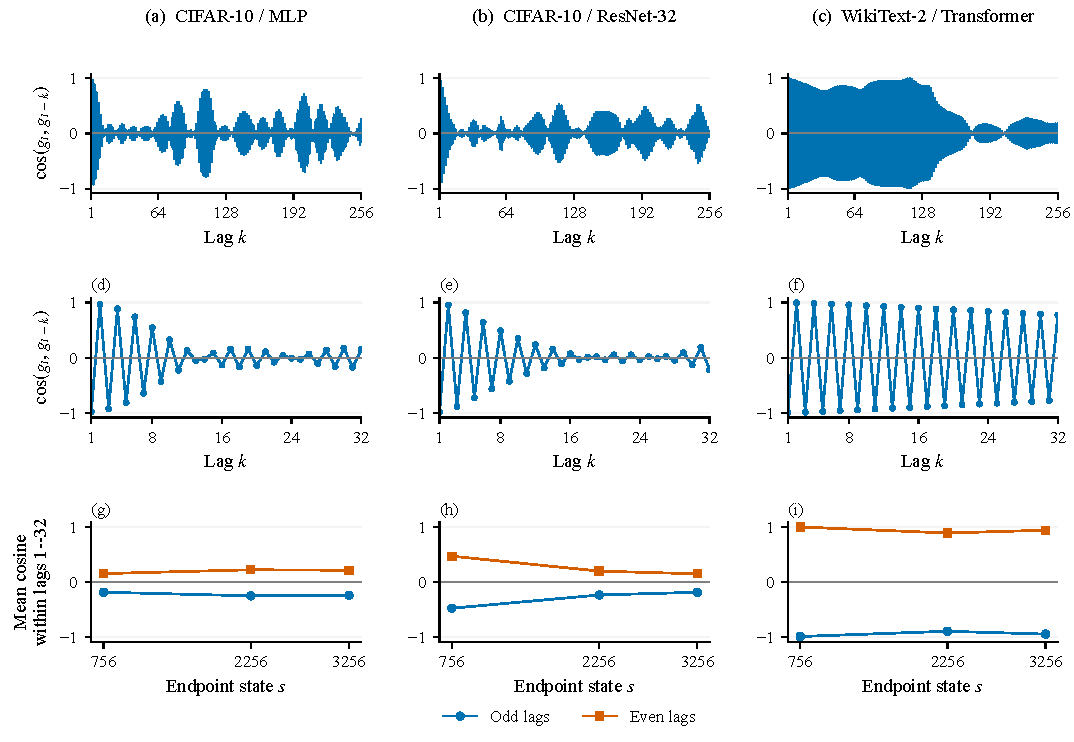
\includegraphics[width=\textwidth]{figures/analysis056/gd_lag_endpoints.pdf}
  \caption{\textbf{Recurring reversal at three sampled endpoints.}
  Top: exact backward cosine $\cos(g_t,g_{t-k})$ at fixed endpoint
  $\theta_{2256}$ ($t=2257$), for lags 1--256.
  Middle: the same values for lags 1--32.
  Bottom: separate odd/even means within lags 1--32 at states
  756, 2256 and 3256; connecting lines guide the eye.
  Rates are 0.04 (MLP), 0.1 (ResNet) and 0.2 (Transformer).
  Each profile comes from a separate 256-update GD continuation
  from saved state 500, 2000 or 3000, with one initialization.
  Exact products use complete raw gradients with FP64 reductions;
  no smoothing or endpoint averaging is applied.
  Later floating-point paths may differ from the original GD runs.
  Alternating correlations describe temporal structure; net movement
  also depends on gradient magnitudes.}
  \label{fig:gd-backward}
\end{figure*}

\begin{figure*}[!t]
  \centering
  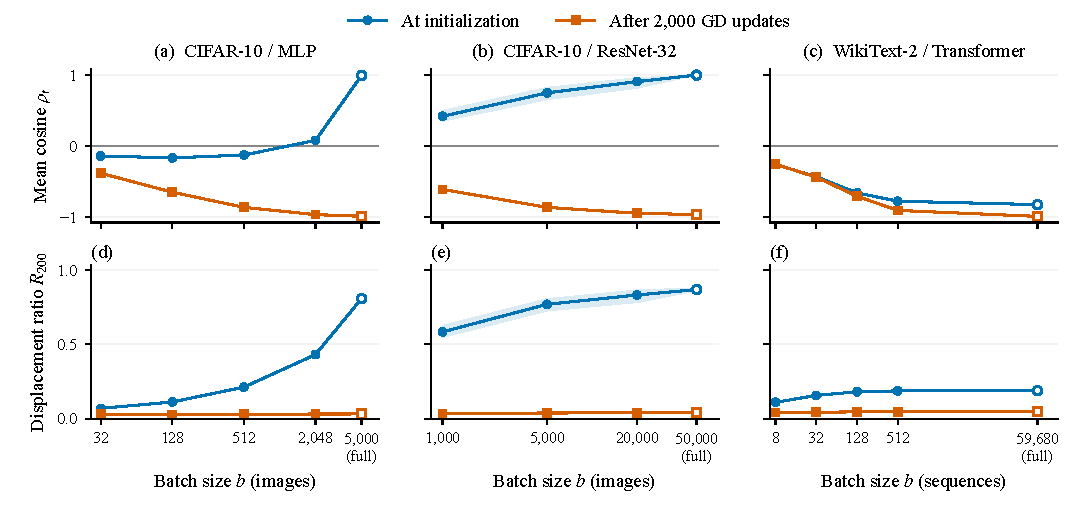
\includegraphics[width=\textwidth]{figures/analysis037/sgd_batch_size_compact.pdf}
  \caption{\textbf{Batch-size dependence of observed alignment during SGD.}
  Mean sampled-gradient cosine over 199 adjacent pairs in 200 updates.
  Blue circles start at initialization; orange squares start after
  2,000 GD updates. The reference trajectories and continuations use
  rates 0.02, 0.1 and 0.2 for MLP, ResNet and Transformer.
  Each line averages eight stochastic repetitions within initialization,
  then weights three initialization blocks equally; shading is their range.
  Hollow rightmost markers denote one full-GD control per block.
  ResNet batches contain whole fixed 1,000-image normalization groups;
  Transformer batches count prepared sequences. Batch axes are logarithmic.
  Parameters evolve during each continuation, so the comparison includes
  both sampling variability and changes in the visited states.}
  \label{fig:sgd-moving-geometry}
\end{figure*}
